% !TeX root = ../main.tex
\chapter*{2. Materials and Methods}
\setcounter{chapter}{2}
\addcontentsline{toc}{chapter}{2. Materials and Methods}
\noindent
In our study, we reconstructed the framework in \citet{guzman2022accounting} (Fig. \ref{fig:framework}b) and illustrated the application values by the empirical data. We created the simulated metacommunity data, as in \citet{guzman2022accounting}, by the process-based metacommunity framework proposed by \citet{thompson2020process} with model parameters regulating the strength of \DIFaddbegin \DIFadd{different }\DIFaddend ecological processes. A simulated metacommunity contained multiple patches, \DIFdelbegin \DIFdel{referring to }\DIFdelend \DIFaddbegin \DIFadd{referred as }\DIFaddend multiple local communities or plots. The three model parameters in \citeauthor{thompson2020process}'s framework, namely niche width, dispersal ability and competition type of the species, are related to the relative importance of environmental filtering and stochasticity, strength of dispersal limitation and different density-dependent biotic \DIFdelbegin \DIFdel{interaction }\DIFdelend \DIFaddbegin \DIFadd{interactions }\DIFaddend underlying the metacommunity. We retained beta-diversity variation partitioning and replaced the hierarchical modeling of species communities (HMSC) considered in \citet{guzman2022accounting} by incorporating two alternative analytical methods: Stegen's framework \citep{stegen2013quantifying} and \DIFaddbegin \DIFadd{the }\DIFaddend dispersal-niche continuum index \citep{vilmi2021dispersal}. We used the random forest (RF) approach to predict the model parameters in \citeauthor{thompson2020process}'s model by using \DIFaddbegin \DIFadd{the }\DIFaddend summary statistics derived from the three analytical methods as predictors. The performance and the robustness of the trained RF were evaluated by calculating the correctness of the prediction and the sensitivity test on sampling effect and time steps selection. To illustrate the application of \citeauthor{guzman2022accounting}'s framework, we considered the observational data from the repeated census of woody plant species in Fushan Forest Dynamics Plot in Taiwan and applied \citeauthor{guzman2022accounting}'s framework to disentangle the ecological processes underlying the Fushan plot. In our study, the symbols in the formulas were mostly consistent with the original papers and we have not attempted to harmonize them. All the simulations and calculations were done in \texttt{Julia} \citep{bezanson2017julia} or \texttt{R} \citep{R}.


%%%%% simulation
\section{Thompson \textit{et al.}'s process process-based metacommunity simulation model}
\label{sec:thom}
%%% a
\subsection{Configuration of the metacommunity simulation model}
\noindent
% reason to use a process-based model
Inference of the underlying ecological processes and the evaluation of the integrated analytical methods were based on the process-based metacommunity framework proposed by \citet{thompson2020process}. \DIFdelbegin \DIFdel{Metacommunity }\DIFdelend \DIFaddbegin \DIFadd{Here, metacommunity }\DIFaddend dynamics is assumed to be a discrete-time model, including three main mechanisms: (1) density-independent abiotic response, (2) density-dependent biotic interactions, and (3) dispersal. In addition, demographic stochasticity is also considered in this model. Niche width, competition types and dispersal ability of the species are the model parameters that modify the strength of these mechanisms and further regulate the strength of the ecological processes. Rigorously, the narrow niche width of the species indicates large fitness difference among species, which increase the strength of environmental filtering in forming the species composition within the local community; the wide niche width of the species results in similar fitness among species, which conversely increases the stochasticity within a local community. Different competition types of species regulate the level of similarity in resource usage, priority effect or competitive hierarchy. Different strength in the dispersal ability of the species indicates different level of dispersal limitation for the species within the metacommunity. These three model parameters are assumed to be independent of each other. 

% Thompson's framework
The framework of \citet{thompson2020process} modeled multiple populations of different species in multiple patches. The population size of the species $i$ in patch $x$ at time $t$ ($t$-th iteration) is denoted by $N_{ix}(t)$. They considered the discrete-time model
\[
N_{ix}(t+1) = N_{ix}(t)\dfrac{r_{ix}(t)}{1+\sum_{j = 1}^S\alpha_{ij}N_{jx}(t)} + I_{ix}(t) - E_{ix}(t)
\]
where 
$r_{ix}(t)$ is the density-independent growth rate of species $i$ in patch $x$ at time $t$, $\alpha_{ij}$ is the per capita effect of species $j$ on species $i$, $S$ is the total number of species, $I_{ix}(t)$ is the number of individuals of species $i$ arrive at patch $x$ from elsewhere in the metacommunity via dispersal at time $t$, and $E_{ix}(t)$ is the number of individuals of species $i$ leave from patch $x$ at time $t$ via dispersal.



%%% b
\subsection{Parametric space in the metacommunity simulation model}
\noindent
% environment
This metacommunity framework assumes that the discrete patches within the metacommunity are linked by dispersal of the species. The patches are located on the torus with equal height and width to avoid edge effect, and the x and y-coordinates of the patches are randomly generated by uniform distribution between 1 and 100. Multiple individuals and different species may co-occur within a patch. The distance matrix of the patches is calculated by the Euclidean distance on the torus. The emigration rate and immigration rate are related to the distance matrix of the patches. The further the patches are, the fewer immigrants the patches produce (see \hyperref[Modelc]{next section} for detailed explanations). The spatial autocorrelated environmental condition of the patches is embedded in the simulated metacommunity. The value describing the state of environmental conditions in each patch (hereafter called environment value) is generated by the stationary isotropic covariance model (by \texttt{RMexp()} function in the \texttt{RandomFields} \texttt{R} package, \citealp{schlather2015analysis}). For each patch, only one environment value \DIFaddbegin \DIFadd{ranging between 0 and 1 }\DIFaddend is generated. Contrary to \citet{thompson2020process}, in our study, the environment value was set to be constant and not fluctuated across time but varied across space with positive spatial autocorrelation. The environment value directly influences species' fitness and further causes the variation in species composition  (see \hyperref[Modelc]{next section} for detailed explanations).

% species
For each species, the species trait, analogical to niche optima, is generated by a random value from a uniform distribution between 0 to 1. The species are assumed to have the same niche width $\sigma$, which controls the relative importance of environmental filtering and stochasticity in forming the species composition within a patch. The species are also assumed to have the same dispersal ability $a$, controls the strength of dispersal limitation.

%%% c
\subsection{Modeling ecological processes in the metacommunity simulation model}
\noindent
\label{Modelc}
% density-independent response
The density-independent per capita growth rate of species $i$ in patch $x$ at time $t$ depends on the niche of species $i$ and the environment value in patch $x$, which is defined as 
\[
r_{ix}(t) = r_{max}\exp(-\frac{(z_i-env_x)^2}{4\sigma^2})
\] 
where $r_{max}$ is the maximum growth rate, $z_i$ is the species trait (niche optima) of species $i$, $env_x$ is the environment value in patch $x$ and $\sigma$ is the niche width of every species. $r_{max}$ was set to be 5 in the simulation.

% competition
The competition parameter ($\alpha_{ij}$) is defined as the per capita impact of species $j$ on species $i$. Five scenarios were considered: (1) no competition ($\alpha_{ii}=1$ and $\alpha_{ij}=0$) (2) equal competition ($\alpha_{ii}=1$ and $\alpha_{ij}=\alpha_{ii}$), (3) stabilizing competition ($\alpha_{ii}=1$ and $\alpha_{ij}\sim Unif[0,0.5]$), (4) Mixed competition ($\alpha_{ii}=1$ and $\alpha_{ij}\sim Unif[0,1.5]$) and (5) competition-colonization trade-off. In case of competition-colonization trade-off, one-third of the species are assigned to be the dominant species which are assumed to impose more impact on inferior species ($\alpha_{ij}\sim Unif[1,1.5]$ and $\alpha_{ji}\sim Unif[0,1]$ if species $j$ is a dominant species and species $i$ is an inferior species). The impact from the same types of species, e.g. one dominant species impacts on another dominant species, is lower ($\alpha_{ji}\sim Unif[0,1]$). 

% dispersal
The number of emigrants $E_{ix}(t)$ of species $i$ from patch $x$ at time $t$ is generated by the binomial distribution where the parameter $n$ is the number of individuals of species $i$ in patch $x$, and the parameters $p$ is the dispersal ability of species \DIFdelbegin \DIFdel{$a$}\DIFdelend \DIFaddbegin \DIFadd{$i$}\DIFaddend . The number of immigrants is determined by the distances between patches on the torus and the number of emigrants from the patches. Suppose the distance between patch \DIFdelbegin \DIFdel{$i$ and patch $j$ is $d_{ij}$}\DIFdelend \DIFaddbegin \DIFadd{$x$ and patch $y$ is $d_{xy}$}\DIFaddend . The expected number of emigrants from patch $y$ immigrating to patch $x$ is defined as 
\[
I_{exp,iyx} = E_{iy}\dfrac{\exp(-0.1d_{xy})}{\sum_{x \neq y}^M \exp(-0.1d_{xy})}
\]
where $M$ is the total number of patches. Thus, the expected total number of immigrants to patch $x$ is equal to the total number of emigrants from other patches $y$ to patch $x$ 
\[
I_{exp,ix} = \sum_{y \neq x} I_{exp,iyx} =  \DIFdelbegin %DIFDELCMD < \dfrac{\sum_{y \neq x} E_{iy}\exp(-0.1d_{xy})}{\sum_{x \neq y}^M \exp(-0.1d_{zy})}
%DIFDELCMD < 	%%%
\DIFdelend \DIFaddbegin \DIFadd{\sum_{y \neq x}}\dfrac{E_{iy}\exp(-0.1d_{xy})}{\sum_{x \neq y}^M \exp(-0.1d_{xy})}
\DIFaddend \text{ , or }
I_{exp} = ED
\]
where $D$ is the dispersal matrix with non-diagnal elements $D_{xy} = \dfrac{\exp(-0.1d_{xy})}{\sum_{x \neq y}^{M} \exp(-0.1d_{xy})}$ and diagonal elements = 0, and $E$ is the emigration matrix with entries $E_{ix}$.The expected total number of immigrants of species $i$ is equal to the total number of emigrant of species $i$: 
\[
I_{exp,i} = 
\sum_{x = 1}^M I_{exp,ix} = 
\sum_{x = 1}^M \sum_{y \neq x}^M \frac{E_{iy}\exp(-0.1d_{xy})}{\sum_{x \neq y}^{M} \exp(-0.1d_{xy})} = 
\sum_{y = 1}^M \frac{E_{iy} \sum_{x \neq y}^M \exp(-0.1d_{xy})}{\sum_{x \neq y}^{M} \exp(-0.1d_{xy})} =
\sum_{y = 1}^M E_{iy}
\]
The number of immigrants of species $i$ to patch $x_1,\dots,x_M$ is generated by the multinomial distribution with probability $(I_{exp,ix_1}/I_{exp,i},\dots,I_{exp,ix_M}/I_{exp,i})$ and $n$ equals to the total number of emigrants of species $i$. The number of immigrants of species $i$ to patch $x$ at time $t$ is denoted as $I_{ix}(t)$. In the case of competition-colonization trade-off, the number of emigrants of the dominant species (weak colonizers) is assumed to be less than the one of the inferior species (strong colonizers). That is, the dispersal ability $a$ of dominant species is 0.1 times the dispersal ability of inferior species.

\begin{figure}
	\centering
	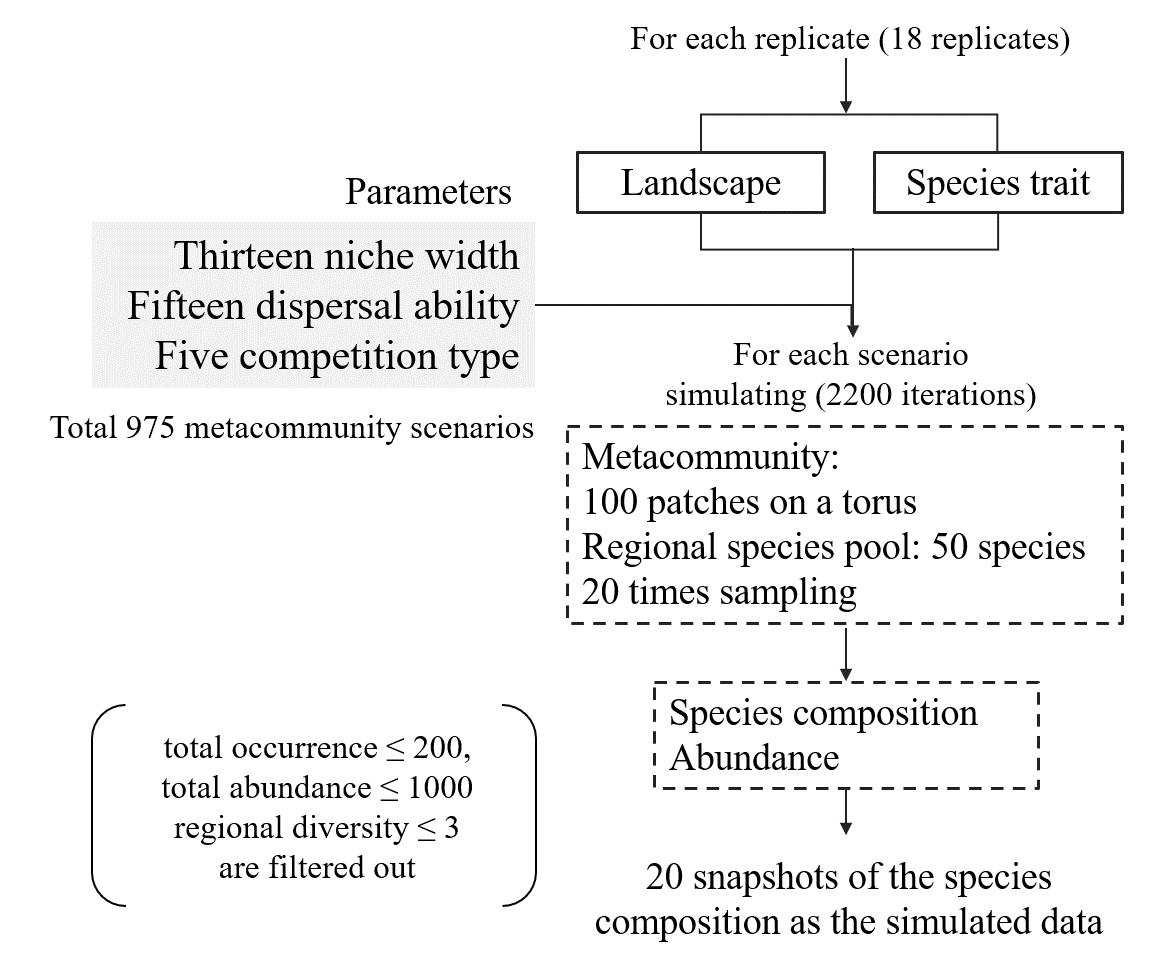
\includegraphics[width=0.7\linewidth]{./figures/ppt/Thompson.png}
	\caption[Flow diagram of process-based metacommunity framework in \citet{thompson2020process}.]{\small
		Flow diagram of process-based metacommunity framework in \citet{thompson2020process}. For each replicate, the coordinates and the environment of the patches, and the trait of species are independently generated before the iteration. The niche width, competition types and dispersal ability of the species are the parameters that regulated the ecological processes underlying the simulated metacommunity. After 2200 iterations, the simulation model generates maximally 100 nonempty patches on a torus. The regional species pool contains maximally 50 species. After the 1800th iteration, every 20 iterations we records the species composition and abundance of the species in each patch. Overall we get 20 snapshots of the species composition from a simulated metacommunity.}
	\label{fig:thompson}
\end{figure}


%%% d
\subsection{Simulation of metacommunity data \DIFaddbegin \DIFadd{with stochasticity}\DIFaddend }
\noindent
For each replicate of the simulation, the landscape configuration, including the coordinates of the patches and the environment value of each patch, and species trait are first generated before the iteration starts (Fig. \ref{fig:thompson}). The environment value in each patch is fixed across all the iterations. The initial species abundance of each species in each patch is generated independently by Poisson distribution with mean 0.5. The simulation ran 2200 iterations, with 200 iterations for the burn-in stage. Within the burn-in stage, the recruitment event, which adds individuals with numbers independently generated by Poisson distribution with mean 0.5 for each species in each patch, is implemented every 20 iterations. The number of individuals of species $i$ in patch $x$ in time $t$ ($t$-th iteration) is denoted by $N_{ix}(t)$. Then, the expected individual number of species $i$ in patch $x$ in time $t+1$ is defined as 
\[
N_{exp,ix}(t+1) = N_{ix}(t)\dfrac{r_{ix}(t)}{1+\sum_{j = 1}^S\alpha_{ij}N_{jx}(t)} - E_{ix}(t)+I_{ix}(t)
\]
The number of individuals of species $i$ in patch $x$ at time $t+1$ is generated by Poisson distribution with mean equal to the expected individual number at time $t$, i.e. $N_{ix}(t+1)\sim Poisson(N_{exp,ix}(t+1))$. After 1800 iterations, the abundance for each species in each patch was recorded until \DIFdelbegin \DIFdel{iteration }\DIFdelend \DIFaddbegin \DIFadd{simulation }\DIFaddend ended for every 20 iterations. We eventually recorded 20 snapshots of the species composition and abundance of a simulated metacommunity ($t = 1,2,...,19,20$) (Fig. \ref{fig:thompson}). 

For each replicate, we simulated the metacommunity dynamics with the same parameters setting proposed by \citet{thompson2020process} (Fig. \ref{fig:thompson}). Thirteen values for niche width $\sigma$ were selected from 0.001 to 10. Fifteen values for dispersal ability $a$ were selected within 0.00001 to 1. The competition type was specified from one of the five scenarios mentioned in the \hyperref[Modelc]{previous section}. Eighteen replicates were run independently.

For further analysis, the samples with low species occurrence, diversity and abundance, i.e. total occurrence $\leq$ 200, total abundance $\leq$ 1000 or regional diversity $\leq$ 3, were excluded. Then, four metacommunity archetypes were defined subjectively by \DIFdelbegin \DIFdel{the }\DIFdelend \DIFaddbegin \DIFadd{a }\DIFaddend specific combination of parameters in the parametric space. \textit{Patch dynamics} (PD) was defined as the one with competition-colonization trade-off and arbitrary determined niche width and dispersal ability; \textit{species sorting} (SS) were defined as the scenario in species with relatively narrow niche width, intermediate dispersal ability and stable competition; \textit{neutral dynamics} (ND) were defined as the one with relatively wide niche width, intermediate dispersal ability and no competition; \textit{mass effect} (ME) was defined as the one with relatively strong dispersal ability, narrow niche width and stable competition. These archetypes represented the extreme scenarios of the simulated metacommunity. They were the samples for testing the effect of the sampling effort and were also used for visualizing the dynamics of the summary statistics. The simulation in this section was run in \texttt{Julia} \citep{bezanson2017julia}.

%%%%% variation partitioning
\section{Beta-diversity variation partitioning}
\noindent
\label{sec:VP}
%%% a
%\subsection*{(a) Introduction: data inputs}
Beta-diversity variation partitioning is a popular method for quantifying the relative importance of environmental filtering and dispersal underlying species turnover. This method was proposed by \citet{borcard1992partialling} and has been widely used in ecological studies \citep{cottenie2005integrating, peres2006variation, smith2010variation}. The method is based on the constrained ordination technique, which quantifies the variation in species composition explained by environment and distance between plots. Species composition, environmental data and geographical information for each plot in the observed metacommunity are needed for this analytical method. The explained variation of environment and space may be further used to compare the relative importance of environmental filtering and dispersal in species turnover across metacommunities \citep{cottenie2005integrating}. However, several issues of variation partitioning have already been discussed \citep[chap.~4]{leibold2017metacommunity}. For example, the more complete the environmental data is, the higher may be the variation explained by the environment, which may even change the inference on which process is the most important \citep{chang2013better}. Another example is that the magnitude of the total variation of species composition may increase when the regional species pool is larger \citep{kraft2011disentangling}. In this case, with the fixed environmental and geographical variables, the unexplained variation of the species composition is expected to increase by chance \citep[pp.~124]{leibold2017metacommunity}.

%%% b
%\subsection*{(b) Analyzing procedure: CCA + dbMeM}
We calculated the summary statistics of beta-diversity variation partitioning for the simulated data generated in \autoref{sec:thom}. Canonical correspondence analysis (CCA) was considered in our study since we assumed that the response of the species to the environment in the simulation model is a Gaussian curve, not a linear line \citep{ter1986canonical, legendre2012numerical}. A snapshot of the species abundance matrix was assigned as the response variable, while environment values generated at the beginning of the simulation and spatial attributes derived from the coordinates of the patches were used as the explanatory variables in CCA. The spatial attributes were derived from applying distance-based Moran's eigenvector maps (dbMEM) on the distance matrix of the patches \citep{borcard2002all}. To quantify the pattern of positive autocorrelation in species abundances, only the eigenfunctions with positive eigenvalues were considered as the explanatory variables. The adjusted R-squared (adjusted R$^2$) \citep[pp.~633]{legendre2012numerical} derived from the variation partitioning in CCA represented: (1) variation explained only by the environment, fraction [a], (2) variation explained only by space, fraction [c], (3) variation explained by both environment and space, fraction [b], and (4) unexplained variation, fraction [d] (Fig. \ref{fig:VP}). We defined fractions [a], [b], [c] and [d] as the summary statistics of beta-diversity variation partitioning. These four partitions of variation were calculated by following: (1) fraction [a]+[b] is the adjusted R$^2$ with species composition as response variable and only environment as explanatory variable in CCA; (2) fraction [b]+[c] is the adjusted R$^2$ with species composition as response variable and only eigenfunctions corresponding to positive eigenvalues as explanatory variables in CCA; (3) fraction [a]+[b]+[c] is the adjusted R$^2$ with species composition as response variable and both environment and eigenfunctions corresponding to positive eigenvalues as explanatory variables in CCA; (4) fraction explained only by environment [a] is calculated by ([a]+[b]+[c])-([b]+[c]); (5) fraction explained only by space [c] is calculated by ([a]+[b]+[c])-([a]+[b]); (6) fraction explained by both environment and space [b] is calculated by ([a]+[b]+[c])-[a]-[c]; (7) unexplained fraction [d] is calculated by 1-([a]+[b]+[c]). All the calculation in this section was done in \texttt{R} \citep{R}.

\begin{figure}
	\centering
	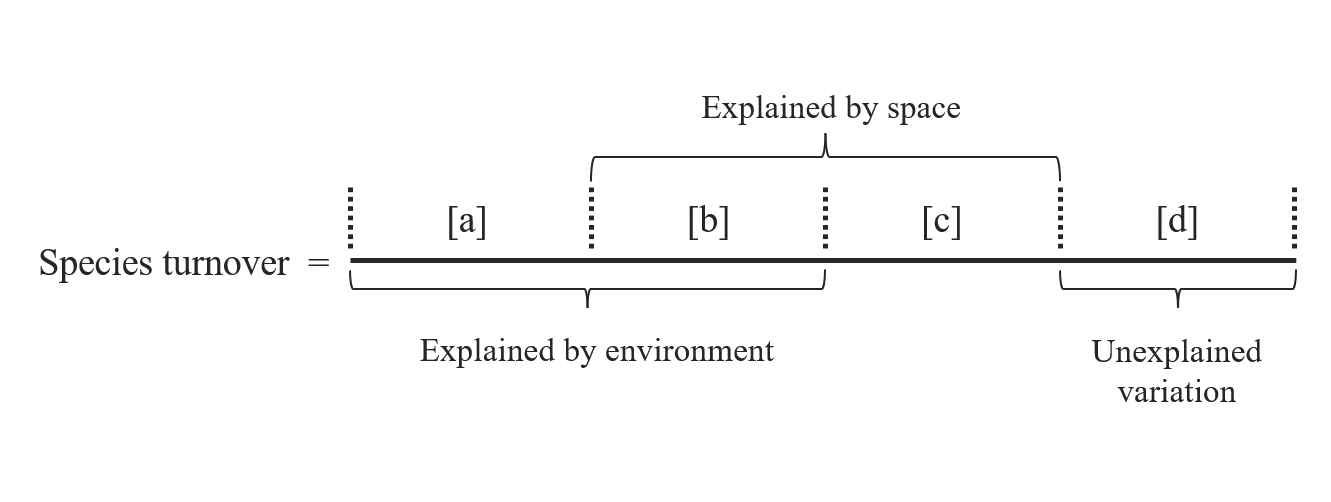
\includegraphics[width=\linewidth]{./figures/ppt/VP.png}
	\caption[Visualization of the statistics of beta-diversity variation partitioning.]{\small
		Visualization of the statistics of beta-diversity variation partitioning (modified Fig. 1 from \citealp{peres2006variation}). Fraction [a] represents the variation explained only by the environment, fraction [b] represents the variation explained only by space, fraction [c] represents the variation explained by both environment and space, and fraction [d] represents the unexplained variation. These four fractions are defined as the summary statistics of beta-diversity variation partitioning. See \autoref{sec:VP} for a detailed explanation.}
	\label{fig:VP}
\end{figure}

%%%%% Stegen
\section{Stegen's framework}
\noindent
\label{sec:Stegen}
%%% a
%\subsection*{(a) Introductions: data inputs}
\citet{stegen2013quantifying} is a null model-based method proposed to quantify the relative importance of selection, dispersal limitation, homogenizing dispersal and drift underlying the microbial metacommunity. Phylogenetic data and species composition data of the observed metacommunity are required in this framework. Compared to most of the null model-based methods that can only disentangle the presence of some ecological processes \citep{ulrich2010null, chase2011disentangling}, \citet{stegen2013quantifying} applied two-step null model to every pair of \DIFdelbegin \DIFdel{the }\DIFdelend plots within the metacommunity. The significance of the divergence or the convergence of the phylogeny structure and species composition between the two plots was tested. The relative importance of the four ecological processes is summarized by the significances derived from all pairs (Fig. \ref{fig:stegen}). \citet{ford2020functional} modified Stegen's framework and used community-level functional trait data instead of phylogenetic data to quantify the relative importance of selection in the fish metacommunity. In our study, we used the trait-based modified version of Stegen's framework proposed by \citet{ford2020functional}.

\begin{figure}
	\centering
	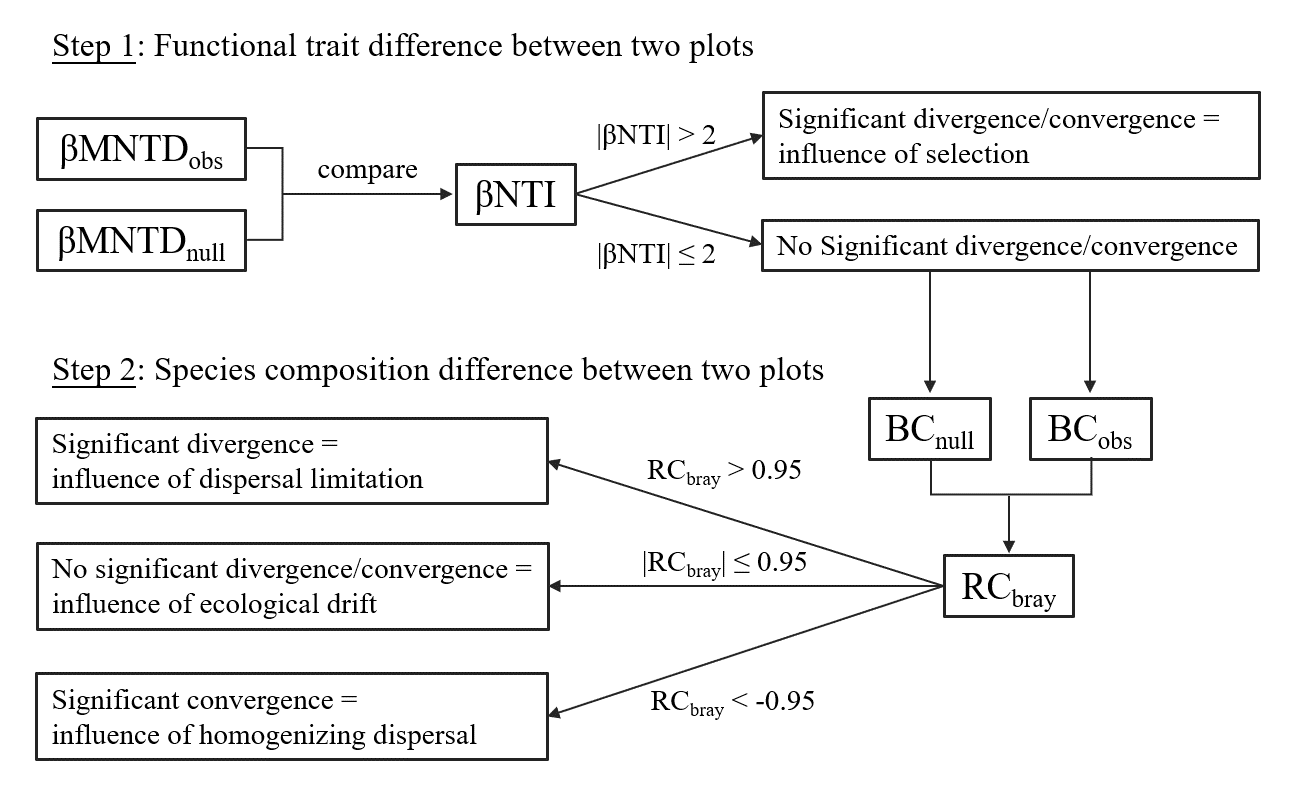
\includegraphics[width=\linewidth]{./figures/ppt/Stegen.png}
	\caption[Flow diagram of modified Stegen's framework of two-step null model.]{\small
		Flow diagram of modified Stegen's framework of two-step null model (modified Fig. 3 from \citet{stegen2013quantifying}). The relative importance of selection, dispersal limitation, ecological drift and homogenizing dispersal underlying the metacommunity are quantified based on the differences in functional traits and species composition between plots. These four values are defined as the summary statistics of modified Stegen's framework. See \autoref{sec:Stegen} for a detailed explanation.}
	\label{fig:stegen}
\end{figure}


%%% b
%\subsection*{(b) Details of procedures}
% first step
The framework proposed by \citet{stegen2013quantifying} and modified by \citet{ford2020functional} consists of two steps. In the first step, abundance-weighted $\beta$-mean-nearest taxon distance ($\beta$MNTD) quantifies the functional distance between two plots. $\beta$MNTD between plot $k$ and plot $m$ is 
\[
\beta \text{MNTD}_{km} = 0.5\cdot \left[\sum_{i_k = 1}^{n_k} f_{i_k}\min(\Delta_{i_k,m}) + \sum_{i_m = 1}^{n_m} f_{i_m}\min(\Delta_{i_m,k})\right]
\]
where $n_k$ is the number of species in plot $k$, $f_{i_k}$ is the relative abundance of $i_k$-th species in plot $k$ and $\min(\Delta_{i_k,m})$ is the minimum of trait difference between $i_k$-th species in plot $k$ and any species in plot $m$. To calculate the deviation of the observed $\beta$MNTD from the null model expectation, species traits are permuted, and $\beta$MNTD is recalculated by the permuted species traits. After repeating 999 times of permutation and recalculation, $\beta$-nearest taxon index ($\beta$NTI) is calculated by the difference of observed $\beta$MNTD and mean of the null model $\beta$MNTD in the unit of the standard deviation of $\beta$MNTD. If $\beta$NTI is larger than 2 or less than -2, then we conclude that the functional turnover is larger than expected and selection is the main process underlying this pair of plots. If $\beta$NTI is within -2 to 2, then go to the second step.

% second step
In the second step, the modified Raup-Crick probability metric (RC$_{bray}$) of \citet{chase2011disentangling} is applied to identify the most important process from the remaining processes, i.e. dispersal limitation, homogenizing dispersal, or drift. The Bray-Curtis distance between two plots is calculated first, and it is recalculated 999 times after the permutation in species abundance. The total abundance and number of species in each plot and the abundance of the species in the whole metacommunity are consistent in the permutation. The observed Bray-Curtis distance and the set of Bray-Curtis distances generated by the null model are combined and standardized into the range of -1 to 1. The modified Raup-Crick probability metric (RC$_{bray}$) is then the standardized observed Bray-Curtis distance. According to the thresholds introduced by \citet{chase2011disentangling}, if RC$_{bray}$ > 0.95, the main process underlying these two plots is dispersal limitation with drift. If RC$_{bray}$ < -0.95, homogenizing dispersal is the main process. If RC$_{bray}$ is within -0.95 and 0.95, pure drift is acting on the species turnover.

%%% outputs
%\subsection*{(c) Outputs: fractions as the statistics in the further analysis}
In our study, we applied \DIFdelbegin \DIFdel{modified Stegen's framework }\DIFdelend \DIFaddbegin \DIFadd{this twe-step null model }\DIFaddend to all the possible pairs of patches in a simulated metacommunity, and calculated the relative importance \DIFaddbegin \DIFadd{(fraction) }\DIFaddend of selection, dispersal limitation with drift, homogenizing dispersal\DIFaddbegin \DIFadd{, }\DIFaddend and pure drift based on the species composition and species traits. These relative importances were treated as the summary statistics of Stegen's framework. All the calculation in this section was done in \texttt{Julia} \citep{bezanson2017julia}.

% DNCI
\section{Dispersal-niche continuum index (DNCI)}
\noindent
\label{sec:dnci}
% a
%\subsection*{(a) Introductions: inputs}
Dispersal-niche continuum index (DNCI) is another null model-based method that aims to quantify the relative importance of niche and dispersal assembly processes underlying the paleontological community data \citep{vilmi2021dispersal} (Fig. \ref{fig:DNCI}). Only grouped species composition data is required to calculate DNCI. This parsimony benefits understanding the ecological processes underlying the paleontological community, whose environment and functional trait data are difficult to collect. The group can be defined based on any cluster analysis or ordination methods.


%\subsection*{(b) Details of procedure}
To calculate DNCI for the simulated metacommunity, we clustered the patches within the metacommunity into two groups based on Ward's minimum variance method \citep[pp360]{legendre2012numerical}. Then the similarity percentage (SIMPER) of each species in the metacommunity, which indicates the contribution of the species to the overall average dissimilarity (OAD) between two groups of patches, was calculated \citep{clarke1993non}. The contribution of species $i$ to the dissimilarity between patch $j$ and $k$ is defined by \citet{clarke1993non} as the Bray-Curtis dissimilarity between patch $j$ and $k$:
\[
\delta_{jk(i)} = \dfrac{|y_{ij} - y_{ik}|}{\sum_{i=1}^p (y_{ij}+y_{ik})}
\]
where $y_{ij}$ and $y_{ik}$ are the abundance of species $i$ in patch $j$ and patch $k$ respectively; $p$ is the number of species in the metacommunity. The raw contribution of species $i$ to OAD $\overline{\delta_i}$ is defined as the average of the contribution of species $i$ to the dissimilarity between every pair of patches in different groups, i.e.
\[
\overline{\delta}_i = \dfrac{1}{M_1M_2}\sum_{\substack{j \in G_1\\ k \in G_2}}\delta_{jk(i)}
\]
where $G_1$ and $G_2$ are the set of patches in group 1 and group 2, and $M_1$ and $M_2$ are the numbers of patches in group 1 and group 2 respectively. The OAD $\overline{\delta}$ is defined by the summation of the raw contribution of all the species, i.e. $\overline{\delta} = \sum_{i=1}^p \overline{\delta}_i$. Finally, the SIMPER profile is derived from the decreasing ranking of the contribution ratio of the species $\overline{\gamma}_i = \overline{\delta}_i/\overline{\delta}$.

Three null models are implemented to disentangle the effect of niche and dispersal assembly processes. Let's suppose that the species composition is with rows as patches and columns as species. The first null hypothesis is $H_{0d}$: only dispersal assembly processes are driving the species turnover within the metacommunity. Under this null hypothesis, the column sum is constrained, and within each column, the abundances are permuted among all patches independently. Additionally, the sum of the abundances of all the species within each plot is constrained to be nonzero. In this case, the total abundance of each species in the metacommunity is kept constant but there may be a different number of individuals and species in a single patch in every permutation. The second null hypothesis was $H_{0n}$: only niche assembly processes are driving the species turnover within the metacommunity. Under this null hypothesis, the row sum was constrained, and within each row, the abundances were permuted independently. In this case, the sum of the abundances of all species in each patch was kept constant, but the total abundance of any of the species is likely to vary in every permutation. The third null hypothesis is $H_{0dn}$: both dispersal and niche assembly processes are driving the species turnover in the metacommunity. Under this null hypothesis, the species composition matrix was permuted with constrained column sum and row sum. Under each of these three null hypotheses, the species composition matrix was permuted 99 times and the SIMPER profile was recalculated by using the permuted species composition. The permutation with three different types of constraint is implemented by the function \texttt{permatfull()} in package \texttt{vegan} in \texttt{R} \citep{R}. To compare the observed SIMPER profile with each null SIMPER profile, the logarithm of the sum of squared deviations $E$ was calculated: 
\[
E = \log_{10}(\sum_{i=1}^p(\overline{\gamma}_{i,null} - \overline{\gamma}_{i,obs})^2)
\]
Finally, for each null hypothesis, we got \DIFdelbegin \DIFdel{100 }\DIFdelend \DIFaddbegin \DIFadd{99 }\DIFaddend $E$ values, which were denoted by $E_{d(q)}$, $E_{n(q)}$ and $E_{dn(q)}$, for $H_{0d}$, $H_{0n}$ and $H_{0dn}$, and $q$ is the index from 1 to \DIFdelbegin \DIFdel{100. }\DIFdelend \DIFaddbegin \DIFadd{99. }\DIFaddend The standard effect sizes ($SES$) of $E_d$ and $E_n$ are defined as the mean of the standardized $E_d$ and $E_n$:
\[
SES_d = \frac{1}{Q}\sum_{q=1}^Q \dfrac{E_{d(q)} - \overline{E}_{dn}}{\sigma_{dn}} = \frac{1}{Q}\sum_{q=1}^Q SES_{d(q)}
\]
\[
SES_n = \frac{1}{Q}\sum_{q=1}^Q \dfrac{E_{n(q)} - \overline{E}_{dn}}{\sigma_{dn}} = \frac{1}{Q}\sum_{q=1}^Q SES_{n(q)}
\]
where $Q$ is the total number of permutations plus one, which is 100, $\overline{E}_{dn}$ is the mean of $E_{dn(q)}$ and $\sigma_{dn}$ is the standard deviation of $E_{dn(q)}$. In the end, the dispersal-niche continuum index (DNCI) is defined as
\[
\text{DNCI} = SES_d - SES_n
\]
and its standard deviation is defined as the squared root of the sum of the square of the standard deviation of the standardized $E_d(q)$ and $E_n(q)$:
\[
\sigma_{\text{DNCI}} = \sqrt{\sigma^2(SES_{d(q)}) + \sigma^2(SES_{n(q)})}
\]
The width of the confidence interval of DNCI is defined as $2\sigma_{\text{DNCI}}$.


% outputs
%\subsection*{(c) Outputs}
DNCI and its standard deviation were used to infer the relative importance of dispersal and niche assembly processes underlying the metacommunity. If DNCI is significantly larger than 0, then niche assembly processes are the dominant processes driving the species turnover. If DNCI is significantly lower than 0, then dispersal assembly processes are the most influential in affecting species composition. If DNCI is not significantly different from 0, then both these two processes may be similarly important for the community assembly. The significance is determined by whether the confidence interval of DNCI encompasses 0. In our study, we treated DNCI and its standard deviation as the summary statistics of the metacommunity. Additionally, since in some cases, the species composition was too sparse (contained too many zeros) and failed to find the column permutation with nonzero row sums, we added the time limitation that if the permutation cannot be found in 30 seconds then we dropped that whole sample. All the calculation in this section was done in \texttt{R} \citep{R}.


\begin{figure}
	\centering
	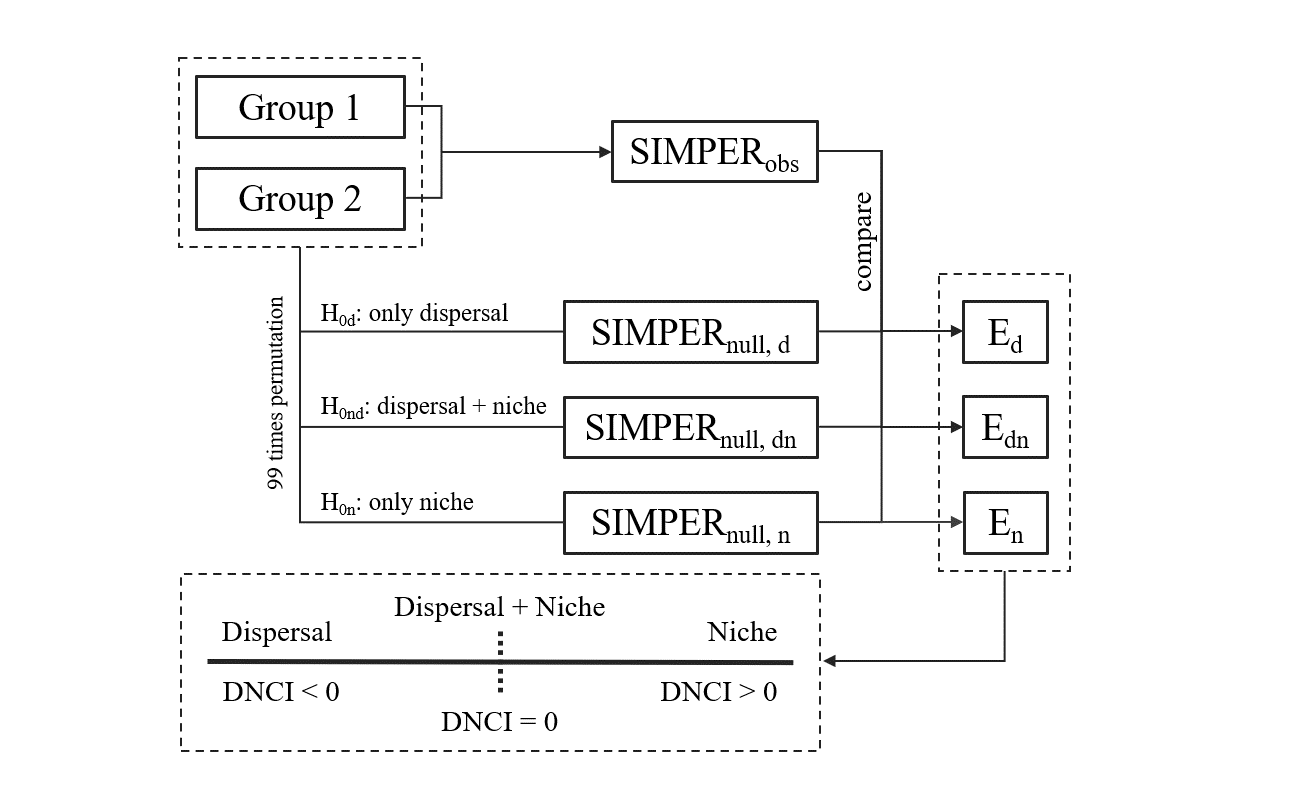
\includegraphics[width=\linewidth]{./figures/ppt/DNCI.png}
	\caption[Flow diagram for calculating dispersal-niche continuum index.]{\small
		Flow diagram for calculating dispersal-niche continuum index (modified Fig. 1 from \citet{vilmi2021dispersal}). By studying the contribution of the species to the dissimilarity within the metacommunity, the relative importance of dispersal and niche assembly processes can be identified by the dispersal-niche continuum index (DNCI). Positive DNCI represents the metacommunity is mainly driven by niche assembly processes; negative DNCI represents the metacommunity is mainly driven by dispersal assembly processes. DNCI and its standard deviation are defined as the summary statistics of these analytical methods. See \autoref{sec:dnci} for a detailed explanation.}
	\label{fig:DNCI}
\end{figure}

%%%%% Random forest
\section{Random forest approach linking summary statistics with parametric space}
\noindent
%%% intro
%\subsection*{(a) Introduction}
Random forest (RF) is a statistical classifier that constructs a mapping between variables by the training data. The correctness of classification and prediction can be quantified by giving the testing data. We applied this statistical approach to construct the link between the summary statistics, which are derived from beta-diversity variation partitioning, Stegen's framework and DNCI, and the model parameters in \citeauthor{thompson2020process}'s process-based metacommunity framework. The trained RF were then applied to the empirical data to disentangle underlying the ecological processes.


%\subsection*{(b) Procedure}
To construct the RF, the first 12 replicates of the simulated data (two-thirds of 18 replicates) were used as the training data and the last 6 replicates of them were used as the testing data. The response variables were the model parameters that influenced the relative importance of ecological processes underlying the metacommunity: niche width, competition type and dispersal ability of the species. Niche width and dispersal ability were treated as ordinal variables \citep{hornung2020ordinal}, and competition type was treated as a categorical variable. We constructed 12 RFs for each model parameter. The explanatory variables of these RFs consisted of four sets of summary statistics and three sets of time steps. We considered the summary statistics derived from only beta-diversity variation partitioning, only Stegen's framework, only DNCI or all three analytical methods with one snapshot ($t = 20$), four snapshots ($t = 20, 16, 12, 8$) or all 20 snapshots of the species composition as the explanatory variables. To evaluate the prediction of the trained RFs, the statistics calculated by the testing data were then entered into the trained RFs, and the accuracy of prediction was estimated by the proportion of the correct link between the prediction of the parameter and the exact model parametric setting. The importance of each explanatory variable, i.e. the statistics derived from the analytical methods, in predicting the model parameters was quantified. For predicting competition type, the importance of the explanatory variables was defined by the mean decrease Gini \citep{han2016variable}, which was derived from the component \texttt{importance} of the object \texttt{randomForest} in \texttt{R}. For predicting niche width and dispersal ability, the importance of the explanatory variables was defined by the permutation variable importance measure \citep{janitza2016random}, which was derived from the component \texttt{varimp} of the object \texttt{ordfor} in \texttt{R}.

Without interpolating, a complete data (with no missing values) is required for constructing and evaluating the RF. Only the samples without missing summary statistics at all 20 periods were used to construct and evaluate the RFs. The missing statistics in some samples at some periods may be caused by the strong stochasticity, which produced the low occurrences, diversity and abundance metacommunities, and the sparseness of the species composition, which resulted in the lack of DNCI.

% sensitivity
\section{Sensitivity analysis to sampling effort and choice of time steps}
\noindent
The robustness of the RFs with summary statistics derived from all three analytical methods at four snapshots to the sampling effort was evaluated. Four archetypes, \textit{species sorting} (SS), \textit{neutral dynamics} (ND), \textit{mass effect} (ME) and \textit{patch dynamics} (PD), were determined by a point in the parametric space defined by dispersal ability, niche width and competition type after the simulation (see \autoref{sec:thom} for details). For the sake of reducing the calculation time, we only considered these four archetypes in the last six replicates as the testing data. We calculated the summary statistics for the four snapshots ($t = 20, 16, 12, 8$) of the simulated species composition generated by the parameters setting of these four archetypes based on the three analytical methods. Then we subsampled the species composition data by randomly choosing 10, 20, ..., and 90 of the patches 15 times independently. For different sampling efforts, the summary statistics were recalculated based on the subsampled species composition and inserted in the trained RF to calculate the accuracy in predicting the model parameters.

We evaluated the robustness of the same RF to the choice of the time steps to be the training data. The explanatory variables of the RF were the summary statistics derived by the three analytical methods from the snapshots at $t = 20, 16, 12, 8$. For each model parameter (niche width, dispersal ability and competition type), we treated the summary statistics at randomly chosen four time steps from $t = 1, 2,\dots, 19, 20$ as the inputs of the trained RF. The correctness of the prediction based on the mismatched summary statistics was calculated. We randomly chose the time steps 1000 times. The distribution of the accuracy for predicting three model parameters was shown in the boxplot.

\section{Application on Fushan Forest Dynamics Plot}
\noindent
The Fushan Forest Dynamics Plot (FDP) is a 25-ha forest dynamics plot established in northern Taiwan in 2004. FDP is located in the subtropical zone at 24˚45'40"N, 121˚33'28"E with elevation from 600 to 733 m.a.s.l. The 500 m x 500 m plot is devided into 625 20 m x 20 m quadrates. The delineation of the plot was conducted in 2002-2003. Precise topography was measured by the electronic total-station theodolites. FDP consists of multiple topographic components, such as hills, ridges, slopes, valleys, flats and creeks. Mean elevation, convexity, slope and aspect of each quadrat were considered as the environmental data of FDP \citep{su2007fushan}. 

The species composition of FDP was surveyed in 2003-2004, 2008-2009, 2013-2014 and 2018-2019, following the method developed by the Center for Tropical Forest Science (CTFS, now ForestGEO) \citep{condit1998tropical}. These four censuses were imagined as the four snapshots of the Fushan forest. All the woody species and the tree ferns with a diameter at breast height (DBH) of $\geq$ 1 cm were identified, measured, mapped and tagged. Within four censuses of FDP, between 111,000 to 134,000 individuals of \DIFdelbegin \DIFdel{114 species in 41 families and 69 }\DIFdelend \DIFaddbegin \DIFadd{111 species in 40 families and 68 }\DIFaddend genera were recorded. Three species of tree ferns, \textit{Cyathea lepifera}, \textit{C. podophylla} and \textit{C. spinulosa} were removed from the further analysis since they are not woody species. The individuals which were missing (status = -1) or lost their stem without DBH of its branches $\geq$ 1 cm (status = -2) were removed from the quadrat in the species composition. Details of the information about environmental conditions and the field survey can be found in \citet{su2007fushan}.

Leaf traits were measured on the randomly selected 6-12 individuals for each species found in the FDP. Specific leaf area (SLA), leaf thickness and leaf dry matter content (LDMC) for 103 specie were obtained based on the established protocols for measuring leaf functional traits \citep{hrguindeguy2013new}. Total organic nitrogen mass per unit leaf mass (N mass) and total organic phosphorus mass per unit leaf mass (P mass) were obtained for 99 of the 103 species based on two microplate methods. The maximum tree height of the 99 species was measured according to the established protocols. The wood density of 74 species was measured in Fushan, of 21 species were obtained from the literature in Taiwan. The wood density of the remaining species was derived from \citet{chave2009towards}.

The species composition, topographical data and coordinates of each quadrat and traits data for each species were used to calculate the summary statistics of beta-diversity variation partitioning, Stegen's framework and DNCI. Since the incompleteness in trait data, when calculating the dissimilarity of traits between two plots in Stegen's framework ($\beta$MNTD), the species with missing traits were ignored. We obtained four sets of summary statistics based on the four snapshots of the species composition in FDP. These summary statistics were inputted into the trained random forest incorporating the three analytical methods and four snapshots with tested performance and robustness to the sampling effort and choice of time steps. Then, the competition types, niche width and dispersal ability of the species in the Fushan forest were estimated.
